\documentclass[12pt,a4paper]{article}

\usepackage[utf8]{inputenc}
\usepackage[T1]{fontenc}
\usepackage{lmodern}
\usepackage[british]{babel}
\usepackage{amsmath,amssymb}
\usepackage{booktabs}
\usepackage{graphicx}
\usepackage[margin=2cm]{geometry}
\usepackage{setspace}
\usepackage{natbib}
\usepackage{hyperref}
\usepackage{tabularx}
\usepackage{array}
\usepackage{tikz}
\usepackage{caption}
\usepackage{nomencl}

\onehalfspacing

\numberwithin{equation}{section}

\bibliographystyle{apalike}

\begin{document}

\pagenumbering{Roman}

% ---- Title Page ----
\begin{titlepage}
\centering
\vspace*{2cm}

{\Large University of Cologne\\[0.3cm]
Faculty of Management, Economics and Social Sciences\\[0.3cm]
Chair in Economics, Energy and Sustainability\\[0.3cm]
Prof.\ Dr.\ Marc Oliver Bettz\"uge}

\vspace{2.5cm}

{\LARGE\bfseries Carbon Leakage through the Back Door?\\[0.4cm]
A Proposed Triple-Difference Design for\\[0.2cm]
EU~ETS Impacts on North African Imports}

\vspace{2.5cm}

{\large Seminar Paper\\[0.3cm]
Panel Data Methods Seminar\\[0.3cm]
Summer Term 2026}

\vspace{2cm}

{\large
Baha Khammari\\[0.2cm]
MSc Economics\\[0.2cm]
Supervisor: Nada Fadl}

\vfill

{\large Cologne, August 2026}

\end{titlepage}

% ---- Abstract ----
\newpage
\section*{Abstract}
\addcontentsline{toc}{section}{Abstract}

The European Union Emissions Trading System (EU~ETS) raises production costs for regulated firms, creating incentives for emission-intensive production to relocate to jurisdictions with weaker carbon pricing. Whether this carbon leakage channel operates through trade flows remains contested: aggregate studies find no measurable effect, yet aggregate estimates may mask corridor-specific leakage into proximate lower-regulation partners. This paper proposes a triple-difference design to estimate the differential semi-elasticity of EU imports of emission-intensive goods from North African partners (Morocco, Algeria, Egypt, Tunisia) with respect to effective EU~ETS carbon costs over 2005 to 2021. The identification strategy exploits variation in product-level carbon-cost exposure, time variation in the effective carbon price attenuated by free allocation, and geographic variation between the North African corridor and a comparison partner group. Product-by-year fixed effects absorb global product-specific shocks; partner-by-year fixed effects absorb macroeconomic and exchange-rate confounds. A positive estimate would indicate that aggregate null results conceal corridor-specific leakage and would sharpen the rationale for the Carbon Border Adjustment Mechanism. A well-identified null in the most leakage-prone corridor would strengthen the interpretation that free allocation has been sufficient to prevent trade diversion.

% ---- Table of Contents ----
\newpage
\tableofcontents

% ---- List of Figures ----
\newpage
\listoffigures
\addcontentsline{toc}{section}{List of Figures}

% ---- List of Tables ----
\listoftables
\addcontentsline{toc}{section}{List of Tables}

% ---- List of Abbreviations ----
\newpage
\section*{List of Abbreviations}
\addcontentsline{toc}{section}{List of Abbreviations}

\begin{tabular}{@{}ll@{}}
CBAM   & Carbon Border Adjustment Mechanism \\
CN     & Combined Nomenclature \\
DiD    & Difference-in-Differences \\
EEA    & European Economic Area \\
EU     & European Union \\
EU~ETS & European Union Emissions Trading System \\
EUA    & European Union Allowance \\
FDI    & Foreign Direct Investment \\
HS     & Harmonised System \\
MSR    & Market Stability Reserve \\
NACE   & Nomenclature statistique des activit\'{e}s \'{e}conomiques \\
NAP    & National Allocation Plan \\
OLS    & Ordinary Least Squares \\
PPML   & Poisson Pseudo-Maximum Likelihood \\
PSM    & Propensity-Score Matching \\
TFP    & Total Factor Productivity \\
\end{tabular}

% ---- Switch to Arabic page numbering for main body ----
\newpage
\pagenumbering{arabic}

\section{Introduction}
\label{sec:introduction}

The European Union Emissions Trading System (EU~ETS), operational since 2005, raises production costs for emission-intensive manufacturers through a cap on aggregate emissions and a market-determined permit price. Standard trade theory predicts that an asymmetric carbon cost shifts comparative advantage toward jurisdictions with weaker regulation and generates \emph{carbon leakage}: an increase in foreign emissions that partially offsets domestic abatement \citep{fowlie2016}. The incentive is strongest for homogeneous commodities traded at common world prices, where regulated producers cannot pass the carbon cost on to buyers and imports substitute for domestic output at the margin. Whether this mechanism operates through trade flows, as opposed to physical relocation, remains an open empirical question. Aggregate studies of EU manufacturing trade find no statistically significant leakage effect \citep{naegele2019}, yet aggregate estimates may mask leakage concentrated in specific bilateral corridors where regulatory asymmetry is large, transport costs are low, and production capacity in emission-intensive sectors already exists.

This paper asks one question: did increases in the effective EU~ETS carbon cost, net of free allocation, raise EU imports of emission-intensive goods from Morocco, Algeria, Egypt, and Tunisia relative to less emission-intensive goods over 2005 to 2021? It proposes and defends a design that would answer it. A positive coefficient would be consistent with the import-leakage channel operating in this corridor. It would not by itself establish physical relocation of production. North Africa is a natural candidate for corridor-specific leakage. The four partners hold Euro-Mediterranean association agreements that established free trade with the EU in industrial goods \citep{eumed}. They host cement, iron and steel, and nitrogen-fertiliser capacity oriented toward export markets, and Egypt ranked fifth among world urea exporters in 2020 \citep{usgs2021}. None of the four priced carbon at any point in the sample period \citep{worldbank2026}. These are precisely the sectors and product categories covered by the Carbon Border Adjustment Mechanism (CBAM; Regulation (EU) 2023/956), which began its transitional phase in October 2023 \citep{cbam2023}. The proposed sample window ends in 2021, before the CBAM proposal could plausibly affect trade patterns, so the design would quantify the pre-CBAM baseline that the mechanism is intended to correct.

The identification strategy rests on a triple-difference specification. Treatment intensity varies across products through their carbon-cost exposure, measured as the CO$_2$ emission intensity of the supplying sector. Treatment varies over time through the effective carbon price, defined as the annual European Union Allowance (EUA) price attenuated by the sector-year free-allocation share. Geographic variation distinguishes the North African corridor from a comparison partner group. Product-by-year fixed effects absorb global product-specific demand and supply shocks, such as Chinese steel overcapacity or commodity-price movements, that are correlated with emission intensity. Partner-by-year fixed effects absorb all time-varying partner-level confounds, including macroeconomic conditions and exchange-rate movements. The triple interaction is therefore identified from the differential response of high-exposure products sourced specifically from lower-regulation partners.

The paper contributes to the empirical literature on carbon leakage in three respects. First, it shifts the unit of analysis from EU-wide averages to a geographically targeted corridor where leakage incentives are strongest. This shift addresses the aggregation concern raised by \citet{verde2020}. Second, it incorporates free-allocation attenuation into the treatment definition, which the firm-level literature typically treats as a robustness dimension. The policy itself used free allocation to mitigate leakage risk \citep{martin2016}. Third, it proposes a pre-CBAM baseline estimate against which the mechanism's effectiveness could eventually be assessed.

The remainder of the paper is organised as follows. Section~\ref{sec:policy} sets out the institutional background insofar as it bears on the treatment definition. Section~\ref{sec:literature} reviews the empirical evidence by mechanism. Section~\ref{sec:design} presents the specification, its identifying assumptions, and the threat each answers. Section~\ref{sec:contribution} discusses what other researchers could take from the design, and Section~\ref{sec:conclusion} concludes.

\section{Policy Background}
\label{sec:policy}

The EU~ETS, established by Directive 2003/87/EC \citep{directive2003}, operates as a cap-and-trade system covering CO$_2$ emissions from power generation and energy-intensive manufacturing across the European Economic Area. Its four phases differ in allocation rules that directly shape the proposed treatment variable (Figure~\ref{fig:timeline}).

\paragraph{Phase~I (2005--2007).}
National allocation plans (NAPs) distributed allowances for free on the basis of historical emissions. Over-allocation was widespread, the EUA spot price collapsed to near zero by mid-2007, and Phase~I allowances could not be banked \citep{ellerman2016}. The effective carbon cost was therefore negligible, a feature the proposed treatment variable captures mechanically.

\paragraph{Phase~II (2008--2012).}
The cap tightened, NAPs underwent stricter Commission review, and banking into Phase~III was permitted. The EUA price reached approximately EUR~25 in mid-2008 before falling to EUR~8 during the financial crisis. Free allocation remained dominant, with auctioning below 4 per cent of allowances \citep{ellerman2016}.

\paragraph{Phase~III (2013--2020).}
EU-wide harmonised rules replaced NAPs. Auctioning became the default for the power sector; manufacturing sectors on the carbon-leakage list received free allocation at product-specific benchmarks set at the 10 per cent most efficient installations. This benchmark-based system introduced cross-sectoral variation in $a_{st}$ independent of installation behaviour, providing the sector-year variation on which the proposed treatment relies. The EUA price remained below EUR~10 for most of 2013 to 2017, partly due to a cumulative surplus of approximately 2 billion allowances.

\paragraph{Market Stability Reserve and price acceleration.}
The MSR, established by Decision (EU) 2015/1814 \citep{msr2015}, began operating in January 2019 and withdrew surplus allowances from circulation. The EUA price rose from EUR~8 in early 2018 to EUR~25 by end-2019 and exceeded EUR~50 in 2021, generating the strongest effective treatment in the proposed sample.

\paragraph{Phase~IV (from 2021) and CBAM.}
The revised Directive tightened the cap reduction factor and reduced free allocation. The proposed sample includes only 2021 from Phase~IV. The Carbon Border Adjustment Mechanism (CBAM), proposed in July 2021 and adopted as Regulation (EU) 2023/956 \citep{cbam2023}, imposes a carbon cost on imports of cement, iron and steel, aluminium, fertilisers, electricity, and hydrogen. Its transitional phase began in October 2023; the definitive regime phases in from 2026 as free allocation is phased out. CBAM's product scope coincides with North African emission-intensive exports to the EU, making this corridor a direct test of the conditions the mechanism addresses. The July 2021 proposal could induce anticipation effects in the final sample year, but anticipation of a border charge deters leakage and would bias the estimated coefficient toward zero. The event-study specification would detect any discontinuous 2021 shift.

\begin{figure}[htbp]
\centering
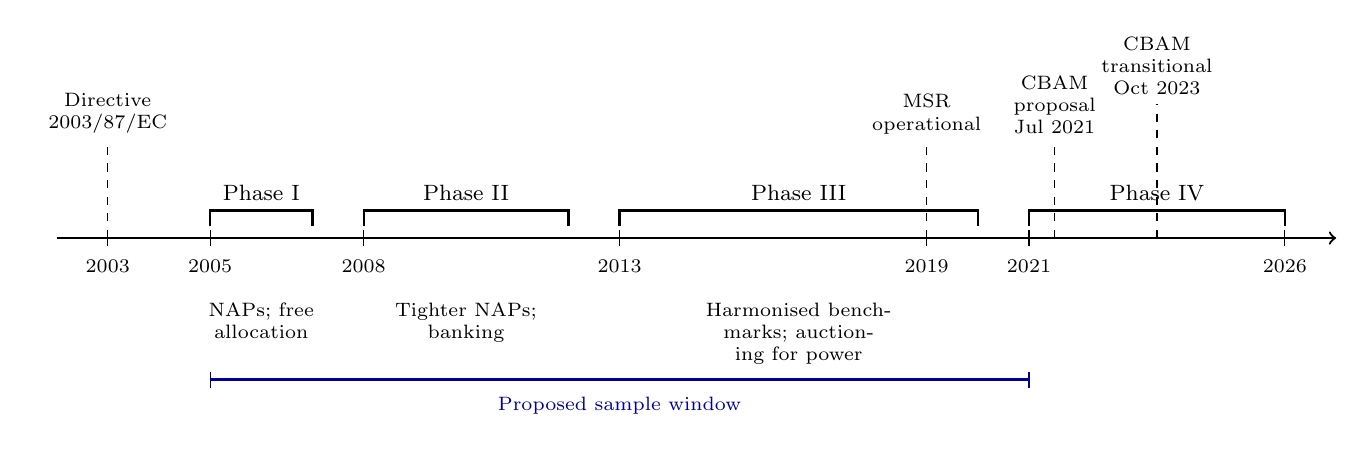
\begin{tikzpicture}[x=0.65cm, y=1cm]

  \draw[thick, ->] (2,0) -- (27,0);

  \draw[thick] (5,0.15) -- (5,0.35) -- (7,0.35) -- (7,0.15);
  \node[above] at (6,0.35) {\footnotesize Phase~I};

  \draw[thick] (8,0.15) -- (8,0.35) -- (12,0.35) -- (12,0.15);
  \node[above] at (10,0.35) {\footnotesize Phase~II};

  \draw[thick] (13,0.15) -- (13,0.35) -- (20,0.35) -- (20,0.15);
  \node[above] at (16.5,0.35) {\footnotesize Phase~III};

  \draw[thick] (21,0.15) -- (21,0.35) -- (26,0.35) -- (26,0.15);
  \node[above] at (23.5,0.35) {\footnotesize Phase~IV};

  \foreach \y/\l in {3/2003, 5/2005, 8/2008, 13/2013, 19/2019, 21/2021, 26/2026} {
    \draw (\y,-0.1) -- (\y,0.1);
    \node[below, font=\scriptsize] at (\y,-0.15) {\l};
  }

  \node[below, font=\scriptsize, text width=1.8cm, align=center] at (6,-0.7) {NAPs; free allocation};
  \node[below, font=\scriptsize, text width=2.2cm, align=center] at (10,-0.7) {Tighter NAPs; banking};
  \node[below, font=\scriptsize, text width=3cm, align=center] at (16.5,-0.7) {Harmonised benchmarks; auctioning for power};

  \draw[dashed] (3,0) -- (3,1.2);
  \node[above, font=\scriptsize, text width=1.8cm, align=center] at (3,1.2) {Directive 2003/87/EC};

  \draw[dashed] (19,0) -- (19,1.2);
  \node[above, font=\scriptsize, text width=1.5cm, align=center] at (19,1.2) {MSR operational};

  \draw[dashed] (21.5,0) -- (21.5,1.2);
  \node[above, font=\scriptsize, text width=1.5cm, align=center] at (21.5,1.2) {CBAM proposal Jul 2021};

  \draw[dashed] (23.5,0) -- (23.5,1.7);
  \node[above, font=\scriptsize, text width=1.8cm, align=center] at (23.5,1.7) {CBAM transitional Oct 2023};

  \draw[very thick, blue!60!black] (5,-1.8) -- (21,-1.8);
  \draw[blue!60!black] (5,-1.9) -- (5,-1.7);
  \draw[blue!60!black] (21,-1.9) -- (21,-1.7);
  \node[below, font=\scriptsize, blue!60!black] at (13,-1.9) {Proposed sample window};

\end{tikzpicture}
\caption{EU~ETS institutional timeline. The four trading phases, key regulatory events, and the proposed sample window (2005--2021). Institutional facts only; no price data plotted.}
\label{fig:timeline}
\end{figure}

\section{Critical Literature Review}
\label{sec:literature}

The empirical literature on EU~ETS carbon leakage divides by mechanism: trade-flow displacement, firm relocation and FDI, and regulated-firm performance. Table~\ref{tab:literature} summarises the identification strategy, data, main finding, and limitation of each study.

\subsection{Trade-Flow Evidence}

\citet{naegele2019} provide the most direct test of trade-flow leakage. They compute trade flows in embodied carbon and in value from Global Trade Analysis Project (GTAP) trade and input-output data over 2004 to 2011, and measure regulatory stringency as the emission cost the EU~ETS imposes on each sector, combining direct and electricity-related indirect costs net of freely allocated allowances. Estimating net-flow specifications with sector-by-country and year fixed effects, alongside bilateral specifications in the spirit of gravity models, they find no evidence that the EU~ETS has caused carbon leakage in European manufacturing. The design's strength lies in its administrative treatment measure and comprehensive sector coverage. Its limitation is aggregation: by pooling all partners and products, it cannot detect leakage concentrated in specific corridors. A separate concern is the sample period, which ends in 2011 and therefore excludes the post-2018 price acceleration.

\citet{aichele2015} estimate the carbon content of bilateral trade among 40~countries over 1995 to 2007, exploiting binding Kyoto commitment as policy variation within a theory-consistent gravity framework. They find that commitment raised a committed country's embodied carbon imports from non-committed partners by approximately 8 per cent and the emission intensity of its imports by roughly 3 per cent, though the binary indicator does not capture carbon-pricing intensity and the sample predates the post-2018 price increase.

\citet{branger2016} study cement and steel, the two most frequently cited leakage candidates, over Phases~I and~II (2005 to 2012). From an analytical model they derive an equation linking EU net imports to domestic and foreign demand and the carbon price, which they estimate with time-series methods. They find no significant effect of the carbon price on net imports of either product and conclude that competitiveness concerns in these sectors have been overstated. The analysis pools all trading partners at the EU level, so it cannot distinguish whether individual bilateral corridors behaved differently from the aggregate, and the sample ends before the Phase~III surplus was absorbed and the MSR took effect.

A common limitation spans all three trade-flow studies: none separates the import-leakage channel by partner-country regulatory stringency. If carbon-cost differentials drive leakage, the effect should be concentrated among partners with no comparable carbon pricing and pre-existing capacity in emission-intensive sectors, precisely the North African corridor this paper targets.

\subsection{Relocation and FDI Evidence}

\citet{koch2019} investigate whether EU~ETS coverage induced German multinationals to shift investment abroad, exploiting the incomplete participation requirements of the system and applying difference-in-differences with bias-corrected matching to the Bundesbank's micro database on outward foreign direct investment (FDI). The average treatment effect on non-EU FDI is close to zero and imprecisely estimated. Two margins qualify this null: less capital-intensive, geographically mobile firms increased their FDI outside the EU by 52 per cent relative to the counterfactual, and regulated firms on average expanded their number of non-EU affiliates by 28 per cent. Relocating firms are neither energy-intensive nor emission-intensive, which limits the scope for actual emissions leakage. The design is credible for the German context but pools destination countries, so it cannot identify whether investment shifted specifically toward lower-regulation partners.

\subsection{Firm-Performance Evidence}

\citet{colmer2025} estimate EU~ETS effects on French manufacturing installations over 2000 to 2012 using one-to-one nearest-neighbour Mahalanobis matching with exact sector matching and a semi-parametric matched difference-in-differences following \citet{heckman1997}. Sector is controlled through the matching procedure, not regression fixed effects. They find emissions reductions of 14 per cent in Phase~I and 16.3 per cent in Phase~II (significant at the 5\% level), emissions-intensity reductions of 17.4 per cent in Phase~II (significant at the 1\% level), and capital increases of 8.3 and 10.5 per cent (significant at the 10\% level). Value added and employment effects are not statistically significant. The pattern is consistent with abatement through capital investment rather than output contraction or relocation.

\citet{dechezlepretre2023} combine installation-level emissions data from France, the Netherlands, Norway, and the United Kingdom with firm-level performance data across EU~ETS countries in a matched difference-in-differences design with a binary treatment indicator. They find emissions reductions of approximately 10 per cent over 2005 to 2012, increases in regulated firms' revenues and fixed assets, and no statistically significant effects on profits or employment. The multi-country coverage strengthens external validity, though the binary treatment indicator does not exploit carbon-cost variation.

\citet{darcangelo2022} estimate effects on total factor productivity (TFP) for Italian manufacturing firms using structural production-function methods and find small, mostly negative effects that are heterogeneous across industries. The finding is inconsistent with a strong Porter-hypothesis interpretation. For the leakage question, the absence of large productivity losses suggests that competitive pressures from EU~ETS regulation have been modest in aggregate.

Surveys by \citet{joltreau2019} and \citet{verde2020} synthesise this evidence and reach similar conclusions: most studies find no significant competitiveness impact, attributing this to generous free allocation, though the predominance of null findings may reflect the weakness of the treatment during the low-price periods covered by most samples.

\subsection{The Gap}

Three features motivate the proposed design. First, trade-flow studies pool all EU trading partners, masking corridor-specific leakage into proximate lower-regulation partners. Second, most samples end before the EUA price exceeded EUR~25 on a sustained basis. The MSR-driven acceleration from 2018 onward remains largely unexamined. Third, free allocation attenuates the very treatment on which most studies rely. \citet{naegele2019} net freely allocated allowances out of their stringency measure, but the firm-level literature typically treats allocation as a robustness dimension rather than a component of the treatment: if free allocation fully offsets the carbon cost, the effective treatment is zero, and failure to account for this attenuation biases the estimated leakage effect toward zero.

\begin{table}[htbp]
\centering
\caption[Summary of empirical studies on EU~ETS carbon leakage]{Summary of Empirical Studies on EU~ETS Carbon Leakage}
\label{tab:literature}
\small
\renewcommand{\arraystretch}{1.3}
\begin{tabularx}{\textwidth}{>{\raggedright\arraybackslash}p{2.8cm} >{\raggedright\arraybackslash}p{2.5cm} >{\raggedright\arraybackslash}p{3.2cm} >{\raggedright\arraybackslash}p{2.8cm} >{\raggedright\arraybackslash}X}
\toprule
Author(s)/Year & Data & Identification & Main Finding & Limitation \\
\midrule
\citet{naegele2019} & Embodied-carbon trade flows, GTAP data, 2004--2011 & Net-flow and bilateral regressions; EU~ETS emission cost net of free allocation & No evidence of trade-flow leakage & Aggregation across partners and products; sample ends 2011 \\
\addlinespace
\citet{aichele2015} & Carbon content of bilateral trade, 40 countries, 1995--2007 & Kyoto commitment in a theory-consistent gravity framework & 8\% higher embodied-carbon imports from non-committed partners & Binary policy indicator; predates the EU~ETS price acceleration \\
\addlinespace
\citet{branger2016} & EU cement and steel net imports, 2005--2012 & Time-series net-import equations with demand controls & No significant carbon-price effect on net imports & EU aggregate; ends before price acceleration \\
\addlinespace
\citet{koch2019} & German multinational outward FDI, Bundesbank micro data & DiD with bias-corrected matching & No average effect; $+$52\% non-EU FDI for mobile, less capital-intensive firms & Pools destination countries; relocating firms not emission-intensive \\
\addlinespace
\citet{colmer2025} & French installations, 2000--2012 & Mahalanobis matching, semi-parametric matched DiD & Emissions $-$14\%/$-$16.3\% (5\% level); capital $+$8.3\%/$+$10.5\% (10\% level) & Single country; ends before price acceleration \\
\addlinespace
\citet{dechezlepretre2023} & Installations in 4 European countries; firm data EU-wide, 2005--2012 & Matched DiD, binary treatment & Emissions $-$10\%; revenues and assets up; no profit or employment effects & Binary treatment; does not exploit carbon-cost variation \\
\addlinespace
\citet{darcangelo2022} & Italian manufacturing firms & Structural production-function TFP estimation & Small, mostly negative, heterogeneous TFP effects & Method-dependent results; no trade-flow dimension \\
\bottomrule
\end{tabularx}
\vspace{0.3em}
\raggedright\footnotesize\textit{Source:} Own compilation based on the cited studies.
\end{table}

\section{Proposed Empirical Design}
\label{sec:design}

This section presents the specifications, defines the treatment, describes the data, and pairs each identifying assumption with its threat and the specification that would probe it.

\subsection{Specification}

The baseline continuous-treatment difference-in-differences, estimated on the North African sample alone, is:
\begin{equation}
\label{eq:baseline}
\ln M_{pct} = \beta \, (\tau_p \times C_{st}) + \phi_{pc} + \psi_{ct} + u_{pct},
\end{equation}
where $M_{pct}$ is the import value (EUR) of product $p$ from partner $c$ in year $t$; $\tau_p$ is product-level carbon-cost exposure; $C_{st}$ is the effective carbon cost of the supplying sector $s = s(p)$; $\phi_{pc}$ are product-by-partner fixed effects; and $\psi_{ct}$ are partner-by-year fixed effects. The preferred triple-difference specification pools the corridor with a comparison partner group:
\begin{equation}
\label{eq:triple}
\ln M_{pct} = \beta \, (\tau_p \times C_{st} \times L_c) + \phi_{pc} + \psi_{ct} + \eta_{pt} + u_{pct},
\end{equation}
where $L_c$ indicates the lower-regulation corridor (Morocco, Algeria, Egypt, Tunisia) and $\eta_{pt}$ are product-by-year fixed effects. A parallel specification would replace $\ln M_{pct}$ with quantity to separate volume from unit-price movements.

\subsection{Variable Definitions}

\paragraph{Carbon-cost exposure ($\tau_p$).}
The CO$_2$ emission intensity of the sector supplying product $p$ under the European industrial activity classification NACE Rev.~2, mapped to products through the RAMON correspondence between the Combined Nomenclature (CN) and NACE \citep{ramon}, fixed at its 2005--2007 average to prevent endogenous intensity responses. The transparent alternative is a binary CBAM Annex~I indicator \citep{cbam2023}.

\paragraph{Effective carbon cost ($C_{st}$).}
\begin{equation}
\label{eq:cst}
C_{st} = P_t \times (1 - a_{st}),
\end{equation}
where $P_t$ is the annual average EUA price \citep{ember} and $a_{st}$ is the sector-year free-allocation share from the EU Transaction Log \citep{eutl}. Free-allocation attenuation is part of the treatment definition: a sector with 100 per cent free allocation faces zero effective cost regardless of the EUA price. An objection is that tradable allowances carry the full permit price as marginal opportunity cost, so lump-sum allocation would leave the output margin unaffected. EU allocation is not lump-sum in this strict sense: activity-level thresholds, closure provisions, and partial-cessation rules tie allowances to continued production, which gives free allocation genuine marginal bite \citep{ellerman2016}. A second concern is mechanical endogeneity: contemporaneous emissions enter the denominator of the allocation share, so demand shocks that cut emissions would raise $a_{st}$ by construction. The baseline therefore computes $a_{st}$ relative to fixed 2005--2007 verified emissions. In Phases~I and~II, $a_{st}$ can exceed one; the baseline caps $a_{st}$ at one. The contemporaneous share and the uncapped version are retained as robustness checks.

\paragraph{Comparison group ($L_c = 0$).}
The choice of comparison group determines what $\beta$ identifies. Three candidates merit consideration. Turkey participates in an EU customs union that eliminates industrial tariffs, so carbon-cost effects are difficult to separate from pre-existing preferential-access effects; Turkey has also begun developing its own emissions trading system, which introduces partial regulatory convergence towards the end of the sample period. The Western Balkans (Albania, Bosnia and Herzegovina, Kosovo, Montenegro, North Macedonia, Serbia) share geographic proximity, operate under Stabilisation and Association Agreements with comparable tariff schedules, and lacked carbon-pricing regimes throughout the sample period, a cleaner regulatory comparison; their limitation is smaller export volumes in emission-intensive goods, which introduces noise. An intra-EU sourcing benchmark would control for EU consumption shocks but faces EU~ETS regulation by construction, so it is not a lower-regulation comparator in the standard sense. The proposed design would report results with each group and discuss sensitivity to this choice.

\paragraph{Fixed-effect absorption.}
In Equation~\ref{eq:triple}, $\eta_{pt}$ absorbs $\tau_p \times C_{st}$, the product-level effect regardless of partner; $\psi_{ct}$ absorbs $C_{st} \times L_c$ and all partner-level macro and exchange-rate shocks; $\phi_{pc}$ absorbs $\tau_p \times L_c$. Only the triple interaction survives. Identification comes from the differential response of high-exposure products from the lower-regulation corridor, purged of global product-specific shocks and partner-specific conditions.

\subsection{Sample and Data}

The sample covers 2005 to 2021, spanning Phase~I through the first year of Phase~IV. Pre-2005 years (2000--2004) are reserved for pre-trend validation; the Directive dates from 2003, so 2000 to 2002 constitutes a clean pre-announcement period and 2003 to 2004 a potential anticipation window. The window ends in 2021 by design: the 2022 energy-price shock, driven by the Russian invasion of Ukraine, distorted both EUA prices and bilateral trade flows in ways unrelated to the leakage channel.

Bilateral trade data at the CN8 level would come from Eurostat Comext (dataset DS-045409; \citealp{comext}), which provides value and quantity by reporting Member State, partner country, product code, and year. Comext coverage of North African partners is comprehensive for goods trade. UN Comtrade data at the six-digit Harmonised System level (HS6) would be the fallback for missing partner-product cells \citep{comtrade}; the coarser classification reduces product-level variation but has wider country coverage. Sectoral CO$_2$ emission intensities would be computed from Eurostat air emissions accounts, defined as tonnes of CO$_2$ per unit of gross output in the corresponding NACE Rev.~2 sector, and mapped to trade products through the RAMON CN-to-NACE correspondence \citep{ramon}.

\subsection{Identifying Assumptions and Threats}

\begin{enumerate}

\item \emph{Parallel trends.} Absent the EU~ETS, differential trends in high-exposure imports from the corridor (relative to comparison partners) would match those for low-exposure products. An event-study specification interacting $\tau_p$ with year indicators (base 2004) would inspect 2000--2002 for pre-trends and 2003--2004 for anticipation.

\item \emph{No confounding product shocks.} Global shocks correlated with emission intensity do not differentially affect the corridor versus comparison partners. $\eta_{pt}$ absorbs all product-by-year variation; a remaining violation would require a shock simultaneously product-specific, intensity-correlated, and corridor-differential. In the baseline Equation~\ref{eq:baseline}, product-level commodity-price controls partially address this.

\item \emph{Carbon-price exogeneity.} The EUA price, set by EU-wide policy and macro factors, is plausibly exogenous to individual bilateral flows. $\psi_{ct}$ absorbs partner-year variation, so identification comes from within-partner-year, across-product variation.

\item \emph{No coincident trade-policy changes.} Euro-Mediterranean association agreement tariff phase-outs could confound the estimate if they coincided with EU~ETS phases and disproportionately affected emission-intensive goods. The agreements entered into force at different dates (Tunisia 1998, Morocco 2000, Egypt 2004, Algeria 2005), and industrial tariff phase-outs were largely completed before the post-2018 price acceleration. The triple-difference mitigates this insofar as comparison partners face similar preferential arrangements.

\item \emph{Over-allocation attenuation.} $a_{st}$ exceeding one in Phases~I and~II mechanically weakens the treatment. Capping $a_{st}$ at one sets $C_{st} = 0$ for over-allocated sector-years; the uncapped version is retained as a robustness check.

\item \emph{CBAM anticipation.} The July 2021 proposal could alter 2021 trade patterns, but anticipation of a border charge deters leakage and biases $\beta$ toward zero. The event-study specification would detect any anomalous 2021 coefficient.

\item \emph{Pandemic disruption.} The years 2020 and 2021 fall within the sample and coincide with severe trade and supply-chain disruption. $\psi_{ct}$ absorbs partner-specific pandemic severity and $\eta_{pt}$ absorbs product-specific demand collapses; a residual violation would require pandemic effects that were simultaneously corridor-specific and correlated with emission intensity. A robustness check would re-estimate the specification excluding 2020 and 2021.

\item \emph{Corridor-specific energy costs.} Algeria and Egypt produce natural gas and regulate domestic energy prices, so the corridor's cost advantage in gas-intensive products widens when European gas prices rise; European gas prices in turn co-move with the EUA price, most strongly after 2018. This confound is corridor-specific, intensity-correlated, and time-varying, so no fixed effect in Equation~\ref{eq:triple} absorbs it. The specification would add a control interacting $\tau_p \times L_c$ with the EU--partner gas-price differential; without this control, $\beta$ would bundle the carbon-cost asymmetry with the energy-cost asymmetry.

\end{enumerate}

\subsection{Inference and Implementation}

Standard errors would be clustered two-way by product and partner-year \citep{cameron2011}. The small number of partner clusters raises finite-cluster concerns; sector-level clustering and a wild cluster bootstrap would address this. The design would be implemented with ordinary least squares (OLS) and high-dimensional fixed effects (\texttt{fixest}; \citealp{berge2021}) and with Poisson pseudo-maximum-likelihood (PPML) estimation (\texttt{fepois}) to handle zero trade flows consistently \citep{santos2006}.

\subsection{Validation}

Two placebo exercises would assess specificity: estimation on non-tradable products for which the import channel is inoperative, and estimation on low-intensity products (below the 25th percentile of $\tau_p$). A heterogeneity analysis would estimate $\beta$ separately for the main CBAM product groups, whose trade exposure differs: cement's low value-to-weight ratio confines trade to short sea routes, which the Mediterranean corridor provides, whereas steel and fertilisers trade globally. Concentration of the effect in products for which corridor trade is feasible would support the leakage interpretation. A positive and significant $\beta$ would be consistent with corridor-specific leakage; a precisely estimated zero would suggest free allocation has been sufficient; an imprecise zero would leave the question unresolved and motivate more disaggregated data.

\section{Contribution and Use to Other Researchers}
\label{sec:contribution}

The proposed design would contribute along three dimensions. First, geographic targeting: existing trade-flow evidence pools all EU partners, so corridor-specific leakage is diluted. By restricting the analysis to North Africa, the design isolates a corridor where regulatory asymmetry is large, transport costs are low, and production capacity in emission-intensive sectors already exists. A positive $\beta$ would indicate that the aggregate nulls documented by \citet{naegele2019} conceal heterogeneity, a finding directly relevant for calibrating CBAM border adjustments by partner country. A well-identified null would carry a different but equally informative implication: that free allocation has been sufficient to prevent trade diversion even where it is most likely.

Second, treatment measurement: by defining the treatment as $C_{st} = P_t \times (1 - a_{st})$, the design measures the carbon cost net of the allocation subsidy, rather than using a binary EU~ETS coverage indicator or the nominal EUA price. This distinction matters: during most of the sample, sectors on the carbon-leakage list received 100 per cent of the benchmark allocation for free, so their effective carbon cost was near zero despite a positive permit price. Studies that treat the nominal EUA price as the treatment overstate cost exposure for these sectors and understate the true treatment contrast across sectors. Researchers estimating competitiveness, innovation, or emissions effects in other contexts would benefit from the same adjustment.

Third, temporal coverage: the MSR-driven price acceleration from 2018 onward generated the strongest effective carbon cost in the EU~ETS's history, yet most existing studies end their samples before 2015. The proposed window through 2021 would test whether leakage effects emerge at higher price levels.

The triple-difference structure, with product-level exposure interacted with a corridor indicator and time-varying policy intensity, is adaptable to other bilateral trade questions where regulation differentially affects product categories and partners. The comparison-group choice, the free-allocation treatment, and the absorption logic are transferable to studies of CBAM effectiveness once the definitive regime generates post-treatment variation.

\section{Conclusion}
\label{sec:conclusion}

This paper has proposed a triple-difference design to estimate whether increases in the effective EU~ETS carbon cost raised EU imports of emission-intensive goods from North African partners over 2005 to 2021. The triple interaction would be identified from the differential response of high-exposure products sourced from the lower-regulation corridor, net of product-level and partner-level time-varying shocks.

The design has limitations. Import flows capture the trade channel of leakage but not physical relocation. A positive estimate would document increased sourcing without establishing that EU production was displaced. The North African corridor accounts for a small share of total EU imports of emission-intensive goods, so external validity to larger partners is uncertain. Third-market export data would separate leakage from diversion on the export side, but partner-side production data, which would confirm that exports reflect expanded capacity, are unavailable at the required disaggregation.

A concrete next step would be to assemble the panel and estimate the specification. The CBAM definitive regime took effect in January 2026. An extension of the panel beyond 2021, drawing on transitional-phase reports from October 2023, would allow estimating whether the border adjustment altered the pre-CBAM pattern.


\newpage
\bibliography{refs}

% ---- AI Acknowledgement ----
\newpage
\section*{Use of AI-Based Tools}
\addcontentsline{toc}{section}{Use of AI-Based Tools}

In accordance with Section~5.2 of the Chair's Guide for Academic Writing (October 2025), the author declares the following use of AI-based tools during the preparation of this paper. Claude (Anthropic) was used for the compilation and formatting of bibliography entries. No AI tool was used for the generation of analytical content, the literature review, or the formulation of the empirical design. The author bears full responsibility for all substantive content.

% ---- Declaration (Eigenst\"andigkeitserkl\"arung) ----
\newpage
\section*{Eigenst\"andigkeitserkl\"arung}
\addcontentsline{toc}{section}{Eigenst\"andigkeitserkl\"arung}

Hiermit versichere ich, dass ich die vorliegende Arbeit selbstst\"andig und ohne die Benutzung anderer als der angegebenen Hilfsmittel angefertigt habe. Alle Stellen, die w\"ortlich oder sinngem\"a\ss{} aus ver\"offentlichten und nicht ver\"offentlichten Schriften entnommen sind, sind als solche kenntlich gemacht. Die Arbeit ist in gleicher oder \"ahnlicher Form noch nicht als Pr\"ufungsarbeit eingereicht worden.

\vspace{3cm}

\noindent
Cologne, \today \hfill Baha Khammari

\end{document}
